\section{任务特定训练方法}
临床实践涵盖多样的认知活动，从主动采集病史到严格提供循证建议。单一训练方式常难以平衡这些场景的不同需求——尤其是诊断所需的演绎逻辑与咨询服务所需的严格事实一致性。为此，我们采用面向不同医学交互形态的任务特定优化策略。本节介绍两项核心能力的专门方法：深度临床问诊（通过分段流水线与带相对基线的逐步惩罚优势算法掌握多轮诊断轨迹）以及可信健康咨询（采用动态量表演化与事实感知强化学习以保证医学信息的安全性与可验证性）。

\begin{figure}[b]
    \centering
    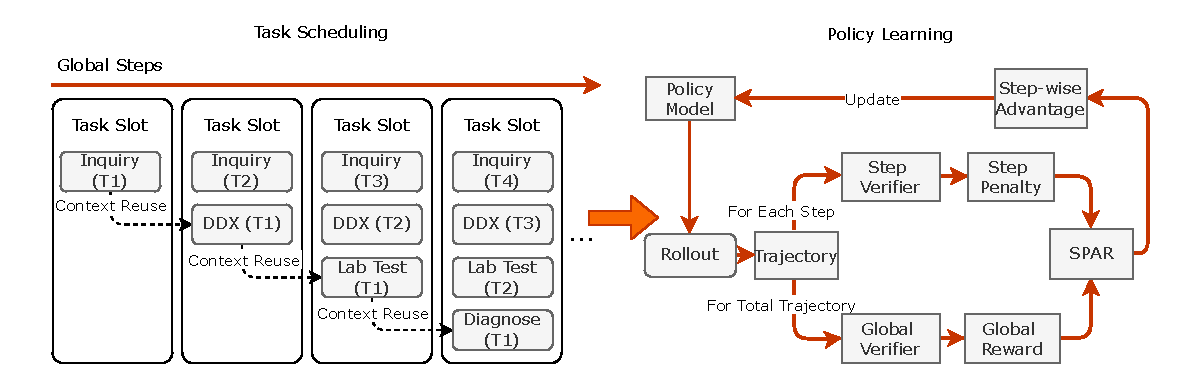
\includegraphics[width=0.98\linewidth]{image/osce.pdf}
    \caption{分段流水线 RL（左）与策略学习算法（右）。}
    \label{fig:spar}
\end{figure}


\subsection{深度临床问诊}
随着医疗 AI 的发展，“基于症状输入的即时诊断”需求迅速上升~\cite{liu2025medchainbridginggapllm}。然而，临床医学远不止简单知识检索，而是建立在严谨证据与演绎逻辑之上的学科。由于相同症状可能源于不同病因且患者个体风险阈值不同，可靠的临床决策必须依赖细粒度数据、系统化风险评估与可追溯推理~\cite{liao2020task, dou2024plpf}。

我们提出深度临床问诊框架，将问诊重新构想为临床级、结构化且可审计的信息生成过程。我们的目标是在简短交互内收集关键临床数据，同时保持严格安全标准。为此，我们提出一套训练框架（见图~\ref{fig:spar}），由分段流水线 RL 架构与带相对基线的逐步惩罚优势（SPAR）算法组成。


\subsubsection{分段流水线 RL}
我们将问诊表述为 $K$ 阶段的生成过程，取 $K=4$。令 $[K]=\{1,\dots,K\}$ 表示阶段索引，$\mathcal{S}=\{\text{Inq},\text{DDX},\text{Lab},\text{Diag}\}$ 为阶段类型集合。
对处于阶段 $k$ 的病例 $i$，用 $x_{k}^{(i)}$ 表示当前输入上下文，包含完整轨迹历史与本阶段指令（例如“基于以上内容，建议检验检查”）。策略 $\pi_\theta$ 生成响应片段 $y_{k}^{(i)}$：
\begin{equation}
    y_{k}^{(i)} \sim \pi_\theta(\cdot | x_{k}^{(i)})
\end{equation}
如图~\ref{fig:spar} 所示，我们采用异步多任务流水线：在全局步 $t$ 上，多个任务槽并行运行于不同流水线阶段（可对应不同病例）；这些阶段特定任务的并集构成训练批次 $\mathcal{B}_t$。

\paragraph{多任务训练目标。}
优化目标是相对于阶段特定目标提升生成片段 $y_k$ 的质量。对一批活跃上下文 $\mathcal{B}_t = \{x_{k_i}^{(i)}\}_{i=1}^N$，联合目标函数为：
\begin{equation}
    \mathcal{J}(\theta) = \frac{1}{|\mathcal{B}_t|} \sum_{x_{k}^{(i)} \in \mathcal{B}_t} \mathcal{L}_{\text{RL}} \left( y_{k}^{(i)}, \mathcal{G}_{k}^{(i)} \right)
\end{equation}
其中 $\mathcal{G}_k$ 为阶段 $k$ 的专属奖励函数。该表述将不同推理能力（信息收集与推导）统一到单一生成模型中。

\paragraph{基于门控迁移的上下文复用。}
流水线依赖自回归的上下文累积。下一阶段输入 $x_{k+1}^{(i)}$ 通过在当前上下文后拼接生成响应 $y_{k}^{(i)}$ 与下一阶段指令 $p_{k+1}$ 构建：
\begin{equation}
    x_{k+1}^{(i)} = [ x_{k}^{(i)}, y_{k}^{(i)}, p_{k+1} ]
\end{equation}
然而，开放式生成存在错误传播风险。为落实“输入垃圾则输出垃圾”的原则，我们实现质量门控迁移。下一阶段的训练池 $\mathcal{D}_{k+1}$ 通过过滤过程填充：
\begin{equation}
    \mathcal{D}_{k+1} \leftarrow 
    \begin{cases} 
        \mathcal{D}_{k+1} \cup \{ [ x_{k}^{(i)}, y_{k}^{(i)}, p_{k+1} ] \}, & \text{if } \mathcal{V}_{k}^{(i)} \ge \tau \\
        \mathcal{D}_{k+1}, & \text{otherwise (Discard)}
    \end{cases}
\end{equation}
其中 $\mathcal{V}_{k}^{(i)}$ 为阶段 $k$ 质量验证器给出的分数，$\tau$ 为接纳阈值。该机制保证只有具有临床有效逻辑链的轨迹被延展，从而有效从训练课程中剪除错误路径。

\subsubsection{策略学习算法：SPAR}
传统 RL 方法（如基于全局奖励的 GRPO~\cite{guo2025deepseek, DBLP:journals/corr/abs-2509-02333}）在长时程医学问诊中存在明显局限，包括奖励欺骗（通过重复提问抬高召回）、逻辑碎片化（临床转移断裂）以及归因无效。在长上下文对话中，轨迹级奖励难以隔离局部错误~\cite{zhang2025lets}，常导致训练不稳定，因为有效推理链会与局部缺陷一并被惩罚。

为解决这些问题，我们提出 SPAR（带相对基线的逐步惩罚优势），引入细粒度的逐步惩罚与解耦的优势估计机制，从而产生自适应课程学习效应。

\paragraph{奖励形式化。}
SPAR 采用层级奖励结构。对于由 $L$ 个逻辑交互步骤 $[z_1, \dots, z_L]$ 组成的生成回复 $y$，我们将每个步骤 $z_j$ 定义为一次完整的对话交换（即用户轮次后接助手轮次）。首先通过预定义临床量表（如诊断准确性、证据完整性）对整条轨迹评估，得到全局奖励 $R_{\text{global}}$。

同时，逐步验证器对每个交互步骤 $z_j$ 进行实时校验。令 $\mathbb{V}_j$ 表示由步骤 $z_j$ 触发的违规类型集合（如冗余、安全风险）。逐步有效性系数 $\gamma_j \in (0, 1]$ 定义为：
\begin{equation}
    \gamma_j =
    \begin{cases}
        1, & \text{if } \mathbb{V}_j = \emptyset \\
        \min\limits_{v \in \mathbb{V}_j} (\lambda_v), & \text{otherwise}
    \end{cases}
\end{equation}
其中 $\lambda_v \in (0, 1)$ 为违规类型 $v$ 的惩罚系数。该形式化遵循最小有效性原则：若某一步出现多种错误，仅施加最严重惩罚（最小 $\lambda$）。该步的有效回报为 $R_j = \gamma_j \cdot R_{\text{global}}$。


\paragraph{逐步优势估计。}
SPAR 的核心创新在于优势计算，将局部惩罚与组内基线解耦。与使用惩罚后分布归一化奖励的传统方法不同，SPAR 通过将\textit{逐步惩罚回报}与\textit{未惩罚组均值}比较来计算步骤 $z_j$ 的优势 $\hat{A}_{j}$：
\begin{equation}
    \hat{A}_{j} = \frac{\gamma_{j} R_{\text{global}} - \mu_{\text{raw}}}{\sigma_{\text{raw}} + \epsilon}
\end{equation}
其中 $\mu_{\text{raw}}$ 与 $\sigma_{\text{raw}}$ 分别为采样组内原始全局奖励（$R_{\text{global}}$）的均值与标准差，不包含任何逐步惩罚。此处采样组指在同一提示（即相同问诊上下文）下生成的多条 rollout，从而支持候选之间的相对比较。

随后我们采用 GSPO 风格的策略更新~\cite{DBLP:journals/corr/abs-2507-18071}，使用逐步优势 $\hat{A}_j$ 加权似然比目标，使惩罚归因于触发违规的具体交互步骤。此处采样组指在同一提示（即相同问诊上下文）下生成的多条 rollout，从而支持候选之间的相对比较。

% We then apply a GSPO-style policy update~\cite{DBLP:journals/corr/abs-2507-18071}, using the step-wise advantages $\hat{A}_j$ to weight the likelihood-ratio objective, so that penalties are attributed to the specific interaction steps responsible for violations.

\paragraph{隐式课程机制。}
该优势设计通过根据错误严重程度自然调度优化优先级，从而形成隐式课程~\cite{bengio2009curriculum}：
\begin{itemize}
    \item \textbf{阶段 1：纠正关键错误。} 对严重违规（如重复），施加严格惩罚（如 $\lambda \approx 0.1$）。这将有效回报 $\gamma_j R_{\text{global}}$ 拉低到显著低于组基线 $\mu_{\text{raw}}$，产生强烈负优势（$\hat{A}_j \ll 0$）。该主导梯度信号促使模型在训练早期优先修复基础可用性问题。
    \item \textbf{阶段 2：细节打磨。} 对轻微瑕疵（如措辞僵硬）采用较轻惩罚（如 $\lambda \approx 0.9$）。初期该微小偏差被全局奖励的高方差（$\sigma_{\text{raw}}$）掩盖；随着策略稳定、$\sigma_{\text{raw}}$ 下降，这些细粒度信号开始主导梯度方向，引导模型向表达质量优化。
\end{itemize}
通过隔离特定步级行为的影响，SPAR 实现精细的归因，将局部缺陷与总体诊断成功区分开来。


\subsection{可信健康咨询}
% 孙
% 可信临床决策
% 临床一致性咨询
本节详细介绍我们面向可信健康咨询的训练方法，聚焦临床可信度与交互效用的融合。为克服静态反馈的局限，我们首先引入动态量表演化框架，以缓解奖励欺骗并确保模型追求真实推理而非表层模式。随后，我们提出事实感知强化学习策略以增强模型的事实推理能力。该方法超越朴素惩罚机制，既能有效抑制不忠实幻觉，又避免诱发保守倾向，从而保持模型提供细致且有信息量的医学建议能力。

\subsubsection{动态量表演化}
在先前工作~\cite{baichuan-m2} 中，我们提出了基于量表的 RL 以提升临床推理能力。但我们观察到该方法容易遭受“奖励欺骗”。模型倾向于追求表层的“高分表现”而非真实推理，表现为被动冗长、模板化防御或臆造细节。其根因在于以往量表仅依赖\textit{输入问题}构建；问题固定后量表静态化，形成可被模型轻易利用的可预测结构。

为解决该问题，我们在 M3 中显著升级反馈信号质量。受 \cite{DBLP:journals/corr/abs-2511-19399,DBLP:journals/corr/abs-2509-21500} 启发，我们提出人机协同的动态演化机制，在量表合成过程中关键性地纳入\textit{模型的响应}。具体而言，我们将约束分为两类：

\begin{itemize}
    \item \textbf{核心量表集合：} 仅基于问题合成，用于引导模型优化总体方向并保证基础安全。
    \item \textbf{动态量表集合：} 基于问题\textit{与}模型历史响应动态合成，用于约束训练过程中发现的不合规行为与具体脆弱点。
\end{itemize}
该动态集合的构建与维护依赖两个关键模块：质量控制与准入/退出规则。

\paragraph{质量控制}
为确保动态生成量表的有效性与临床相关性，我们实现“挖掘-验证-注入”的闭环流程。
首先识别高置信样本——在当前系统下得分高但潜藏缺陷的响应。
随后量表挖掘代理分析这些样本，识别对抗模式并拟定候选约束。
最后由人类专家进行校验。专家无需从零制定规则，而是审核代理输出，评估其边界确定性与元原则一致性（如安全性 $>$ 经验性）。这确保量表激励推理本身，而非转移奖励欺骗的焦点。

\paragraph{准入与退出规则}
为防止规则爆炸并保持奖励信号强度，动态量表集合遵循“问题驱动”的生命周期：

\begin{itemize}
    \item \textbf{准入：} 候选量表并非仅因“正确”而被接纳，只有当其针对统计显著的失败模式（即模型响应中违规率较高）时才会激活，从而保证反馈聚焦于活跃行为缺陷。
    \item \textbf{退出：} 当某约束在多个训练轮次中持续被满足（违规率 $\rightarrow 0$）时，将自动从动态集合中移除。该“剪枝”机制防止奖励信号被稀释，使优化焦点严格聚焦于新出现且未解决的问题，而不被冗余正向奖励冲淡。
\end{itemize}


\subsubsection{事实感知强化学习}
\label{sec:fact-aware}

在带验证奖励的强化学习（RLVR）范式中，朴素的幻觉抑制策略通常将验证信号直接转化为标量惩罚~\cite{DBLP:conf/emnlp/MinKLLYKIZH23, chen2025learning}。标准目标形式定义为：
\begin{equation}
R = R_{task} + \alpha \cdot R_{hallu}
\label{eq:naive-objective}
\end{equation}
其中 $R_{hallu}$ 使用基于计数的幻觉率度量（$-N_{\text{hallu}}/N_{\text{total}}$）。该目标试图在惩罚项降低幻觉的同时保留核心医学推理能力（$R_{task}$），但在长文本生成中容易遭受两种主要的奖励欺骗：

\begin{itemize}
    \item \textbf{冗余稀释：} 模型通过生成大量事实正确但价值较低的陈述来抬高分母 $N_{\text{total}}$，在不修正核心错误的情况下降低测得的幻觉率。

    \item \textbf{惩罚诱导的保守：} 严苛惩罚会促使模型采取过度保守策略（如缩短输出以规避惩罚），从而削弱探索与复杂推理行为的习得。
\end{itemize}
为解决这些问题，我们提出包含结构化信号去噪与动态多目标聚合的联合优化框架，如图~\ref{fig:fact_aware_rl_fig} 所示。

\begin{figure}[t]
    \centering
    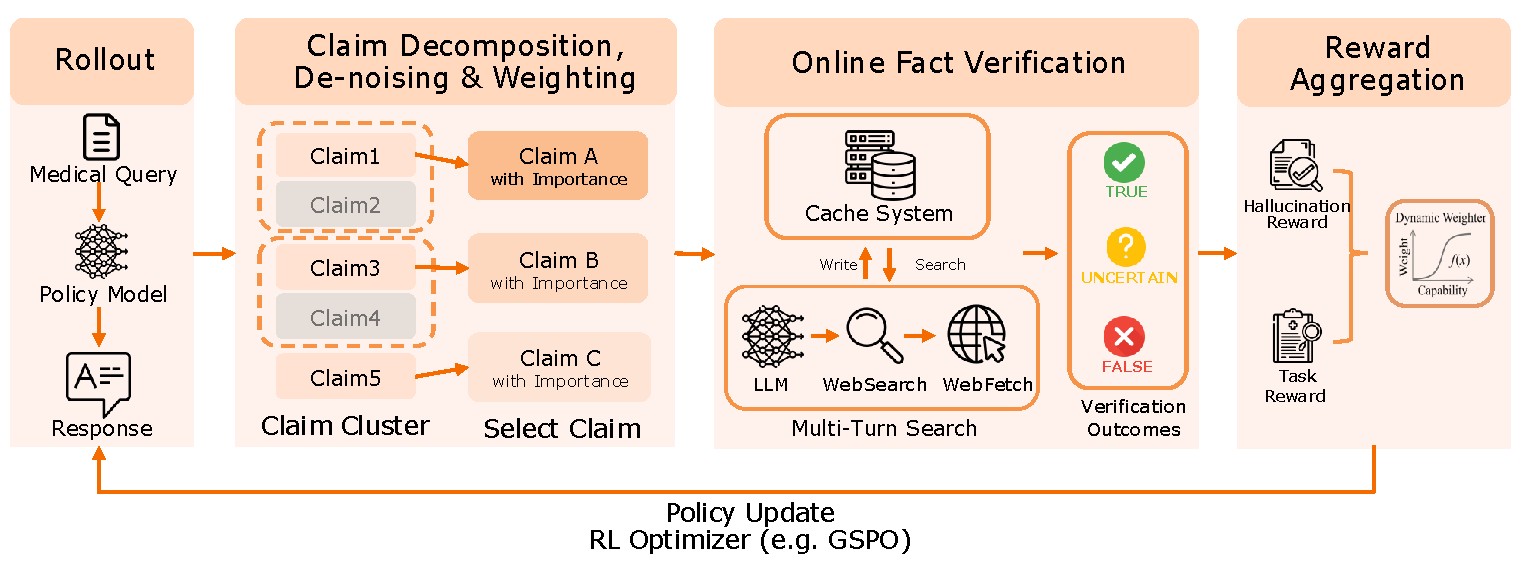
\includegraphics[width=0.98\linewidth]{image/fact-aware-rl.pdf}
    \caption{事实感知强化学习算法。}
    \label{fig:fact_aware_rl_fig}
\end{figure}

\paragraph{结构化信号去噪}

为建立对冗余鲁棒的奖励信号，我们将原子事实的验证重构为基于语义密度的加权评估，确保核心诊断陈述中的幻觉受到显著高于边缘内容的惩罚。

我们首先通过语义编码器 $\mathcal{E}(\cdot)$ 将回复序列 $\{s_j\}$ 与抽取事实 $\{c_i\}$ 映射到向量空间。为防止通过同义改写操纵指标，我们使用余弦相似度阈值进行语义聚类。对每个簇 $\mathcal{C}_k$ 选取代表事实 $c_k^*$，将评估指标从词频转为语义单元密度。随后用显著性权重 $w(c_k^*)$ 量化每条事实的信息贡献，定义为其在回复句子中的最大语义相关性：
\begin{equation}
w(c_k^*) = \max_{1 \le j \le M} \cos(\mathcal{E}_{c_k^*}, \mathcal{E}_{s_j})
\end{equation}
事实性奖励 $R_{fact}$ 计算为加权惩罚项：
\begin{equation}
R_{fact} = - \frac{\sum_{k=1}^{K} w(c_k^*) \cdot \mathbb{I}(c_k^*)}{\sum_{k=1}^{K} w(c_k^*) + \epsilon}
\end{equation}
其中 $\mathbb{I}(c_k^*)$ 为验证惩罚指示函数，定义为：
\begin{equation}
\mathbb{I}(c_k^*) = 
\begin{cases} 
1 & \text{if } c_k^* \in \{\text{Refuted}, \text{Uncertain}\} \\
0 & \text{otherwise}
\end{cases}
\end{equation}
从机制上看，加权分母抵消事实数量膨胀（抗稀释），而依赖显著性的分子确保惩罚集中于核心错误而非边缘文本，从而保留推理效用。

\paragraph{动态多目标聚合}

为平衡医学推理强化与幻觉抑制，我们实现动态聚合机制，引入软门控系数 $\lambda(R_{task})$，根据在策略生成回复上获得的任务奖励调节惩罚强度。

给定特定回复的 $R_{task}$，我们使用成形 Sigmoid 函数将动态系数 $\lambda(R_{task})$ 严格定义为任务奖励的函数：
\begin{equation}
\lambda(R_{task}) = \sigma \left( \kappa \cdot \frac{R_{task} - \mu}{\Delta} \right)
\end{equation}
其中 $\sigma(\cdot)$ 为标准 sigmoid 函数，中心为 $\mu = (\tau_{min} + \tau_{max})/2$，尺度为 $\Delta = \tau_{max} - \tau_{min}$（陡峭度 $\kappa=10$）。

阈值通过对任务奖励分布的后验分析进行校准。我们设定 $\tau_{min} = 0.75$、$\tau_{max} = 0.95$ 以界定反映有效医学推理的关键区间，使惩罚强度与模型能力相匹配：

\begin{itemize}
    \item \textbf{保护区（$R_{task} < \tau_{min}$）：} $\lambda(R_{task}) \to 0$。抑制惩罚以优先优化能力，避免干扰基础推理技能的习得。
    \item \textbf{过渡区（$\tau_{min} \le R_{task} \le \tau_{max}$）：} $\lambda(R_{task})$ 非线性上升，系统逐步引入事实约束。
    \item \textbf{约束区（$R_{task} > \tau_{max}$）：} $\lambda(R_{task}) \to 1$。当模型具备足够推理能力时施加完整惩罚，以最大化幻觉抑制。
\end{itemize}

最终总奖励 $R$ 将任务效用与门控事实惩罚项聚合：
\begin{equation}
R = R_{task} + \lambda(R_{task}) \cdot R_{fact}
\label{eq:full-fact-aware-rl}
\end{equation}
该形式化实现了隐式课程：先保障推理能力，再施加严格安全约束。我们在附录 \ref{sec:ablation_reward} 中通过对比消融实验验证这一行为。

















% \subsection{Other Reasoning Tasks}

% yangfan: 这部分在正文中不重点介绍，medxqa-rubrics 可以在附录中说明
% 需要补充一个实验：纯 RLVR（answer verify） 的 baseline。
% This section introduces the training for Medical QA tasks. 
% MedBullet, M2 General Task
% GRPO, RLVR
